\chapter{State of the art}

In this chapter I will present how things are today in the field of containerization.  I will start with a quick reminder of the difference between virtualization and containerization, then go through some existing solutions for both of those concepts.

\section{Virtualization vs Containerization}
\paragraph{}Both virtualization and containerization aims at providing an abstraction layer that allows the application or the OS located above the abstraction to behave like if he was the only one present on this layer.  The key difference between those two is where this abstraction layer is located.  

\paragraph{}To keep it simple, for the virtualization, the abstraction is between the OS and the hardware, the OS thinks it is running on a baremetal machine but is actually hosted on another machine.  For the containerization, the abstraction is between the appliciation and the OS, the application thinks it is the only one running in the system but it is actually only isolated in its own namespace.  As a good illustration is better than a thousand words, Figure \ref{fig:virt-vs-cont} represents this difference. 
\begin{figure}[!h]
  \begin{center}
    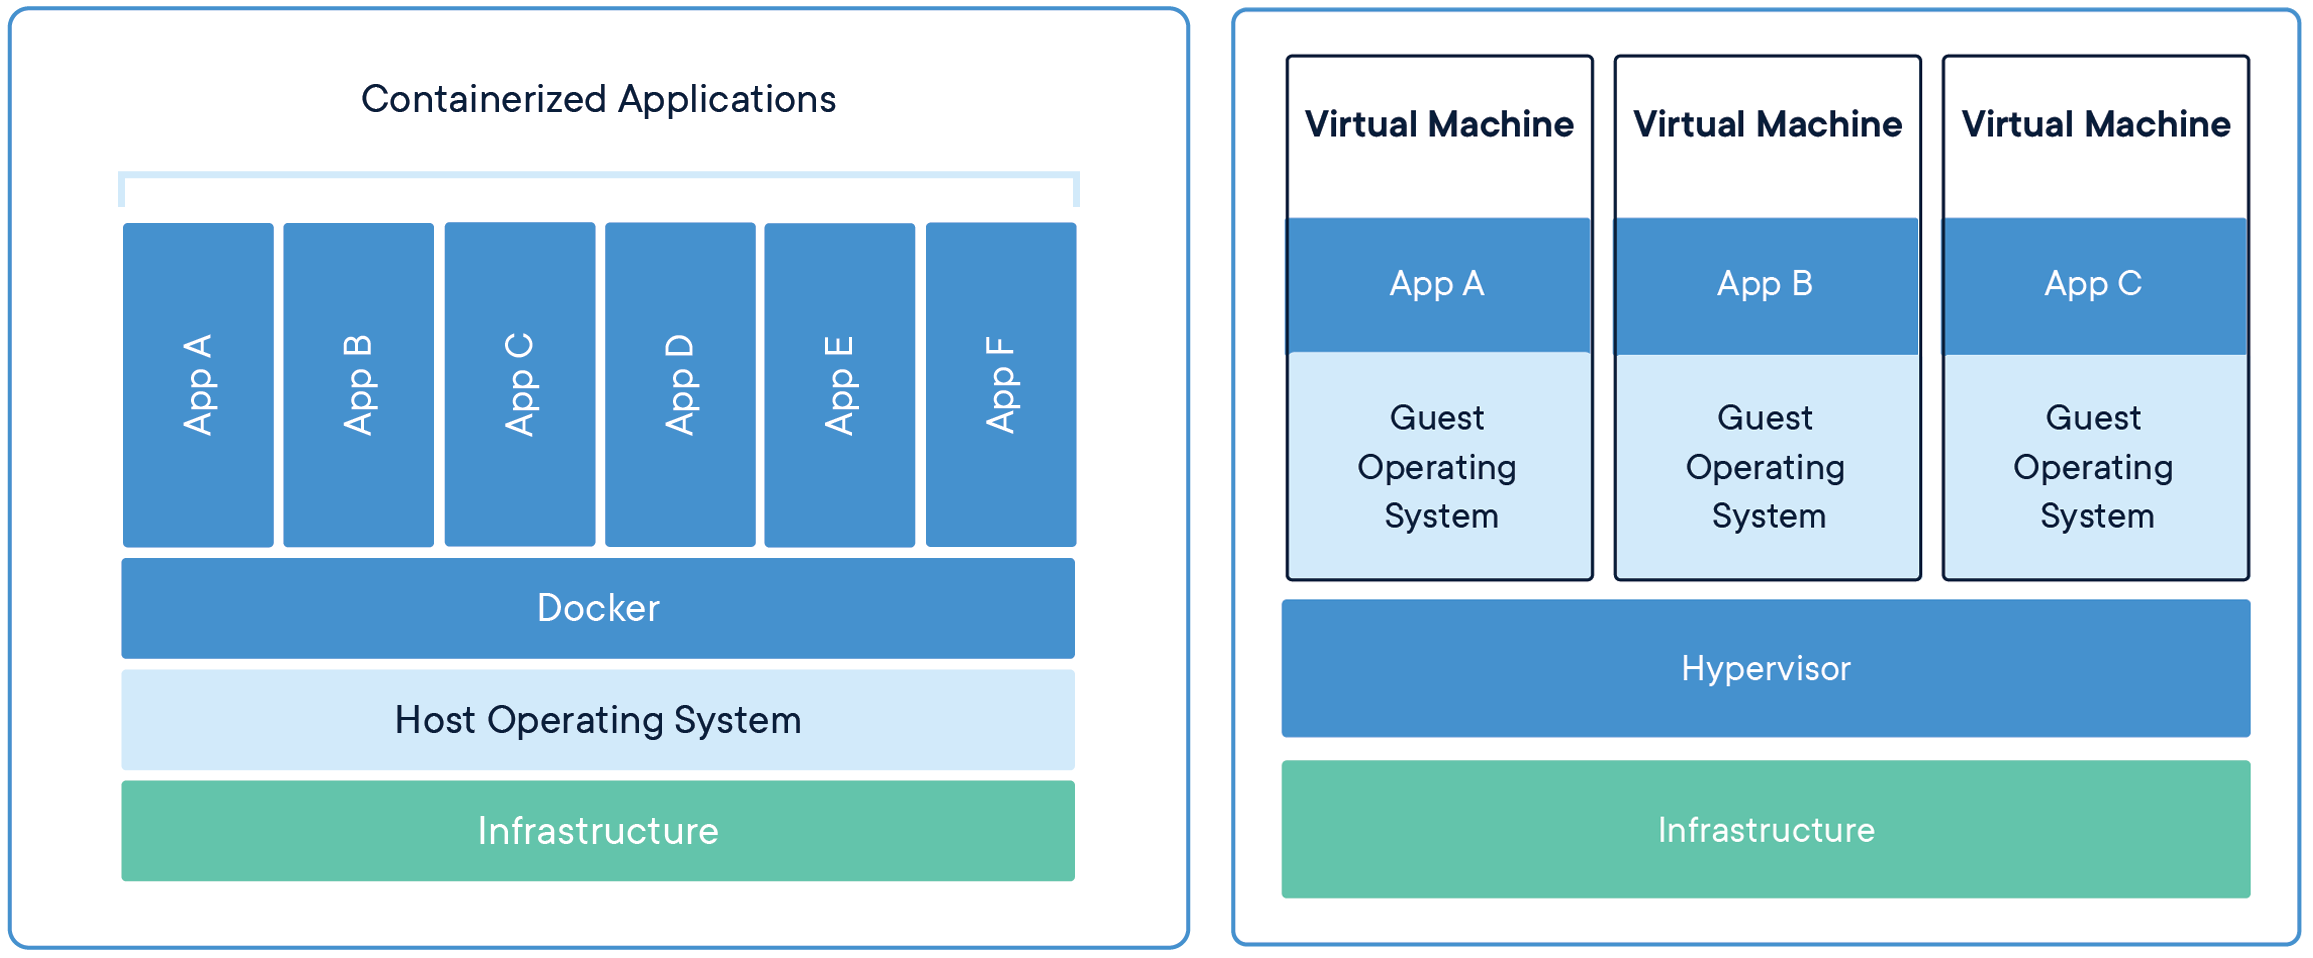
\includegraphics[width=\linewidth]{images/Virtualization-Containerization.png}
    \caption{\cite{docker}}
    \label{fig:virt-vs-cont}
  \end{center}
\end{figure}

\paragraph{}Because of what they are, those two solutions usually didn't apply to the same situations.  A VM (Virtual Machine) is a much more complicated and complete structure, that takes more time to boot but provides a better isolation.  And the Container is much lighter, quicker to launch but less isolated.  Traditionally, in the Cloud Computing world, VM's rely in IaaS (Infrastructure-as-a-Service) while Containers rely in PaaS (Platform-as-a-Service).

\paragraph{}But recently things started to change, some new solutions seem to have the advantage of both sides, the isolation of a VM and the portability and lightness of a Container.  This is why some VM-based solution are presented here.  Even though VMs do not come from the same domain of applciation as Containers, and even though in the case of INGInious, Containers were 5 years ago the obvious choice, it might now be time to reconsider it.

\section{Containerization solutions}
\subsection{Docker}
\subsection{Podman}
\subsection{runC}
\subsection{SAND}
\subsection{SOCK} \cite{oakes2018sock}

\section{Virtualization solutions}
\subsection{Firecracker}
\subsection{Kata Containers}
\subsection{LightVM} \cite{manco2017my}
